A more general way to look at de Bruijn sequence is universal cycle ($U$-cycle). 
\begin{definition}[Universal cycle]
    Given a finite set $\mathcal{T}_{k}$ of distinct of combinatorial objects of "rank $k$", an $U$-cycle of $\mathcal{T}_{k}$ is a cyclic sequence $\cU=(a_0,a_1,\ldots,a_n)$ such that $(a_{i+1},\ldots,a_{i+k})$, $0\leq i\leq n$, run through each element of $\mathcal{T}_{k}$, where index addition is performed modulo $n$.
\end{definition} 
An order $k$ binary de Bruijn sequence is eventually an $U$-cycle of the set of all length $k$ binary strings. The studies of $U$-cycle are concerned in the existence and construction of $U$-cycles for many combinatorial objects such as string, permutations, partitions, subsets, multisets, lattice paths, vector spaces weak orders, etc~\cite{chung1992universal,horan2013universal,jackson2009research,johnson2009universal,hurlbert2009universal,jackson2009recursive}. Section~\ref{subsect:fanchung} provides results for permutations, partitions, ans subsets of a set of $n$ distinct symbols, where $n$ is a positive integers. These results was first summarized by Fan Chung et.al in~\cite{chung1992universal}.
%, for example: the set of all $n!$ permutations of $\left\{1,2,\ldots,n\right\}$, partitions of $\left\{1,2,\ldots,n\right\}$~\cite{chung1992universal}. 

\subsection{Permutations, partitions and subsets of \texorpdfstring{$n$}{n} distinct symbols}\label{subsect:fanchung}
Consider the set $S_{n}$ of all $n!$ permutations of $\left\{1,2,\ldots,n\right\}$. With each value of $n$, set $S_{n}$ may not always contain any $U$-cycles, such as $n=3$. All $6$ permutations of $\left\{1,2,3\right\}$ are $S_{3}=\left\{123,132,213,231,312,321\right\}$, and the longest cycle in $S_{3}$ one can travel is of length $4$, for instance,  $123\rightarrow231\rightarrow312\rightarrow123$, which still lacks $132, 321$. 

However, if order-isomorphism is allowed instead of requiring exact match, $U$-cycles of $S_{n}$ exists. More precisely, an $U$-cycle $U_{n}=(a_{0},a_{1},\ldots,a_{n!-1})$, $a_{i}\in\left\{1,2,\ldots,N\right\}$, for $S_{n}$ is $n!$-tuple such that each element of $S_{n}$ is order-isomorphic to exactly one block $(a_{i+1},\ldots,a_{i+n})$, where $a_{i}=a_{j\equiv i(\mod n!)}$. Here, two $n$-tuples $\bfa=\left(a_{1},a_{2},\ldots,a_{n}\right)$ and $\bfb=\left(b_{1},b_{2},\ldots,b_{n}\right)$ are called order-isomorphic, written as $\bfa\sim\bfb$, if $a_{i}<a_{j} \Leftrightarrow b_{i}<b_{j}$ for all $0<i,j\leq n$. An example of $U$-cycle for $S_{3}$ is :
\[1\ 4\ 5\ 2\ 4 \ 3\]
By order-isomorphism, each $3$-tuple in the above $U$-cycles can be mapped into elements of $S_{3}$ as follow:
\begin{align*}
    145\sim123 \\
    452\sim231 \\
    524\sim312 \\
    243\sim132 \\
    431\sim312 \\
    314\sim213 
\end{align*}
and hence, the equivalent cycle is $123\rightarrow 231\rightarrow 312\rightarrow132\rightarrow312\rightarrow 213\rightarrow123 $. The construction of de Bruijn graph can be imitated to construct the transition graph for $S_{n}$. Each permutation plays the role of a vertex. Their suffix of length $n-1$ is analyzed to establish its edges to other permutations. Takes the vertex $231$ of $S_{3}$ as an example. From its suffix $31$, one can go to $312$. But since order-isomorphism is accepted, and note that $31\sim21\sim32$, there are also edges connecting $231$ to $213$ and $321$. The whole transition graph of $S_{3}$ is shown in figure \ref{fig:S3_graph}.

\begin{figure}[htbp]
    \centering
    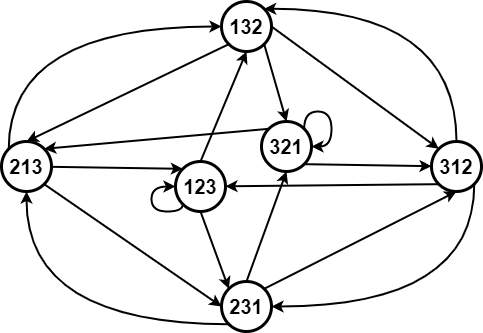
\includegraphics[scale=0.5]{fig/PermutationGraph.png}
    \caption{Transition graph of $S_{3}$.}
    \label{fig:S3_graph}
\end{figure}

It is proved that the transition graph of $S_{n}$ is Hamiltonian, and a Hamiltonian cycle in the transition graph corresponding to an $U$-cycle in $S_{n}$. Now, the key question is how to represent a $U$-cycle of an Hamiltonian cycle, like the sequence $1\ 4\ 5\ 2\ 4\ 3$ represents $123\rightarrow 231\rightarrow 312\rightarrow132\rightarrow312\rightarrow 213\rightarrow123 $. Even with $S_{3}$, is $5$ the smallest number of distinct symbol necessary for an $U$-cycle. More generally, how many distinct symbols does an $U$-cycle of $S_{n}$ use at least? 

Actually, in $S_{3}$, one can do better with $4$ symbols. For example, the sequence $1\ 4\ 2\ 3\ 4\ 2$ is the representation of Hamiltonian cycle:
\[132\rightarrow312\rightarrow123\rightarrow231\rightarrow321\rightarrow213\rightarrow132\]
The following sequence is an example with $5$ symbols for $S_{4}$:
\[1\ 2\ 3\ 4\ 1\ 2\ 5\ 3\ 4\ 1\ 5\ 3\ 2\ 1\ 4\ 5\ 3\ 2\ 4\ 1\ 3\ 2\ 5\ 4 \]
Let $N(n)$ be the minimum number required for an $U$-cycle of $S_{n}$, it is proved that:
\[N(2)=2,\ N(3) = 4,\ N(4)=5\ \mathrm{and}\ n+1\leq N(n)\leq 6n\ \mathrm{for}\ n\geq5\]
Fan Chung believes that the equation happens at $n+1$. However, their belief still remains an unsolved conjecture until now.
\begin{conjecture}
    $N(n)=n+1$.
\end{conjecture}

Constructing transition graph is also help finding $U$-cycle for the set of $P_{n}$ of partitions of the set $\left\{1,2,\ldots,n\right\}$. The partitions can be represented by sequence of length $n$ $(a_{0},a_{1},\ldots,a_{n})$, where $a_{i}=a_{j}$ indicates the $i$-th element and $j$-th element are in the same group of the partition. The transition graph of $P_{n}$ is illustrated in figure~\ref{fig:P3_graph}.

\begin{figure}[htbp]
    \centering
    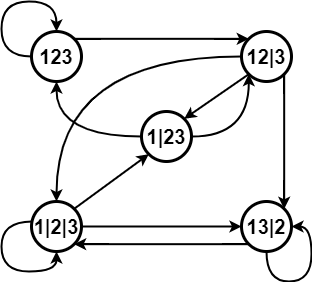
\includegraphics[scale=0.5]{fig/partitions.png}
    \caption{Transition graph of $P_{3}$.}
    \label{fig:P3_graph}
\end{figure}

Transition graph of $P_{n}$ is proved to be Hamiltonian by showing that it can be clustered to be an Eulerian graph. 

It is more challenging to study the family ${n \brack k}$ of all $k$-element subsets of a set of $n$ distinct elements $\left\{0,1,\ldots,n-1\right\}$. This thesis provides an example of an $U$-cycle for case $n=5,k=2$:
\[1\ 3\ 2\ 5\ 4\ 2\ 1\ 5\ 3\ 4\]

The question about the condition for the existence of the universal cycle for such family is still not answered completely. The difficulty here is that a transition graph for ${n \brack k}$ isn't able to be defined explicitly. This issue is caused by the distinguishing feature of an $k$-set. More precisely, a $k$-element subset might occur in any $k!$ possible order in $U$-cycle, but it is only allowed to occur once. Fan Chung and Graham made a conjecture on this problem and the first person who can solve it would earn a prize awarded by author's conjecture .

\begin{conjecture}[Fan Chung's conjecture]\label{conjecture:fanchung}
    Universal cycle for ${n \brack k}$ always exists provided $k$ divides $\dbinom{n-1}{k-1}$ and $n$ is large enough.
\end{conjecture}

It's easy to see that conjecture~\ref{conjecture:fanchung} is true for $k=1,2$. Effort on this question has just cracked completely the cases $k=3,4,5$ (with some aid of a computer), and $k=6$ whenever $n\ \mathrm{and}\ k$ are relatively prime(~\cite{hurlbert1994universal,jackson1993universal}). For $k\geq 7$, and $k=6$ when $n\ \mathrm{and}\ k$ are not relatively prime, conjecture~\ref{conjecture:fanchung} remains open. 

Beside studying the existence of $U$-cycle on different kinds of sets, designing algorithms that create universal cycles are also concerned.
\subsection{Universal cycles algorithms for other classes of sets}
There are researches focusing on using generalized the \gls{fkm} algorithm and greedy algorithm to create universal cycles for a class of sets. Moreno proved that this method works for the set of rotations of the lexicographically largest $i$ necklace~\cite{moreno2004theorem}. The aperiodic strings in the set of all $k$-ary strings of length $n$ can be generated the same way as shown by Au in~\cite{au2015generalized}. All these results is later generalized by Joe Sawada et.al in~\cite{sawada2016generalizing}. More particularly, let $\bfS$ to be the set of length $n$ $k$-ary strings such that the following closure conditions are obeyed:
\begin{itemize}
    \item The set of strings $\bfS$ is closed under rotation.
    \item Its subset of necklaces is closed under replacing any suffix of length $i$ by $k^i$. 
\end{itemize}
Then, the greedy and \gls{fkm} algorithm create the lexicographically smallest universal cycle of $\bfS$. Several such classes $\bfS$ are listed in example~\ref{exp:closed_S}.

\begin{example}\label{exp:closed_S}
Recall that $\Sigma_{q}=\{1,2,3,\ldots,q\}$ is a code alphabet of size $q$, and $\Sigma_{q}^{n}$ is the set of $q$-ary sequences of length $n$ over alphabet $\Sigma$. The following sets satisfy the closure conditions for the existence of universal cycles proved by Sawada~\cite{sawada2016generalizing}.
\begin{itemize}
    \item \textbf{Minimum Sum}: $\bfS\in\Sigma_{q}^{n}$ is a set of length $n$ strings with sum over all of its symbol at least $s$, where $s$ is a given constant.
    \item \textbf{Frequency of $q$}: $\bfS\in\Sigma_{q}^{n}$ contains the strings with at least $l_{q}$ copies of $q$, where $l_{q}$ is a given constant.
    \item \textbf{Frequency of $i<q$}: $\bfS\in\Sigma_{q}^{n}$ contains the strings with at most $u_{i}$ copies of $i<q$. Here, $u_{i}$ is a given constant.
    \item \textbf{Avoiding a substring}: $\bfS\in\Sigma_{q}^{n}$ contains the strings that do not contain a given pattern $\alpha\in\Sigma_{q-1}^{m}$, for some $m\geq1$, as a cyclic substring. 
    \item \textbf{Union and Intersection}: Let $\bfS_{1}$ and $\bfS_{2}$ be $2$ set obeying the closure conditions, then both $\bfS_{1}\cup \bfS_{2}$ and $\bfS_{1}\cap \bfS_{2}$ also satisfy those conditions.
\end{itemize}
\end{example}
Note that, in example~\ref{exp:closed_S}, the union and intersection of the proper sets $\bfS$ allow to combine the previous results to create more interesting classes of sets that have universal cycles. 

Section~\ref{sec:universal_cycles} has provides different research directions and results on universal cycle, which is a generalization of de Bruijn sequences. The applications of de Bruijn sequences and its generalizations will be presented in the next section. 
